\definecolor{roleColor}{HTML}{1F77B4}
\definecolor{skillColor}{HTML}{2CA02C}
\definecolor{responsibilityColor}{HTML}{FF7F0E}
\definecolor{benefitColor}{HTML}{9467BD}
\definecolor{companyBlurbColor}{HTML}{8C564B}
\definecolor{callToActionColor}{HTML}{D62728}
\definecolor{inclusivityColor}{HTML}{7F7F7F}
\definecolor{applicationColor}{HTML}{17BECF}

\newcommand{\legenditem}[2]{\textcolor{#2}{\rule{0.8em}{0.8em}}\hspace{0.5em}\textbf{#1}}

\chapter{Data Cleaning}
\section{Perché il Data Cleaning è necessario}

Come abbiamo visto nel capitolo precedente, gli \textit{embeddings} dei documenti ne rappresentano la \textbf{semantica}. Di conseguenza due documenti di simile significato saranno convertiti in vettori vicini.

I documenti che sono \textbf{vicini} nello spazio semantico e che si trovano in una \textbf{zona densa} di punti vengono quindi inseriti nello stesso cluster. Questo pone due importanti restrizioni nel dataset:

\begin{enumerate}
    \item I documenti devono essere \textbf{semanticamente coerenti}, poiché ogni frase inutile influisce sulla posizione del documento nello spazio semantico; di conseguenza il rumore compromette la \textbf{coerenza dei cluster}.
    \item Le frasi che riguardano argomenti non importanti per lo studio (e.g. stipendi, paragrafi legali, descrizioni aziendali, ecc.), oltre a influire sulla posizione dell'\textit{embedding} nello spazio, creano cluster non utili ai fini dell'analisi, poiché comparendo in quasi tutti i documenti generano zone dense.
\end{enumerate}

Il secondo punto è particolarmente delicato, perché cluster fittizi che raggruppano documenti in base a fattori irrilevanti non solo creano ``topic spazzatura'', cioè non informativi, ma riducono anche la sensibilità ai dettagli distintivi di un documento (e.g. mansioni, abilità richieste), sottraendo ai cluster effettivi documenti importanti.

Per visualizzare l'effetto di un data cleaning accurato confrontiamo il comportamento del modello su un dataset non preprocessato (Figura~\ref{fig:garbage-barplot}).

\begin{figure}[H]
    \centering
    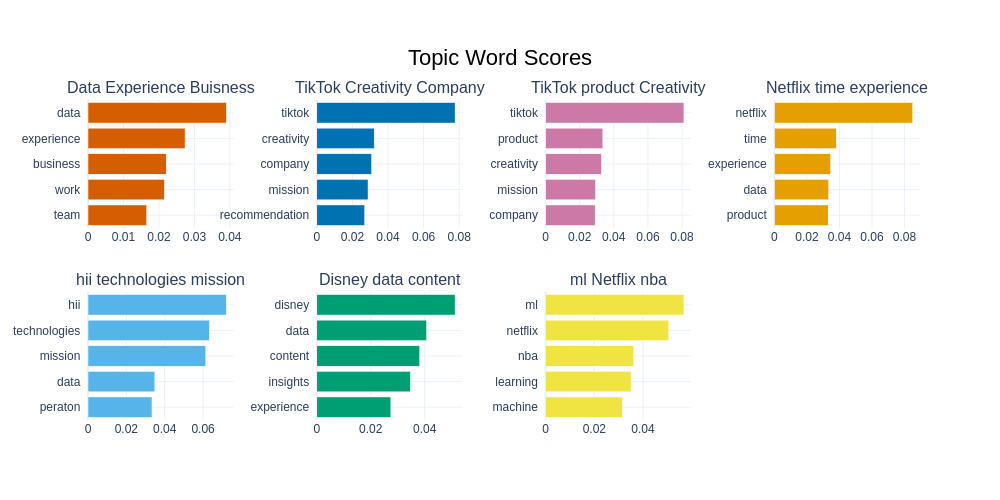
\includegraphics[width=\linewidth]{cleaning/garbage_barplot.png}
    \caption{Barplot ottenuto da \textit{topic modeling} senza \textit{preprocess}.}
    \label{fig:garbage-barplot}
\end{figure}

Come visto nel capitolo precedente, a ogni parola è associato uno \textit{score} che ne rappresenta l'importanza all'interno del topic. Questo barplot ci permette di fare alcune considerazioni importanti sulla natura del dataset e sulla direzione che deve assumere la pulizia dei dati. Innanzitutto notiamo che i nomi delle aziende, come TikTok e Netflix, hanno un peso molto grande; ciò è coerente con la natura del dataset, composto da offerte di lavoro basate negli USA, quindi è plausibile che Big Tech e altre multinazionali compaiano nella maggior parte degli annunci. Altre parole poco informative che compaiono in più topic sono legate al gergo aziendale (e.g. mission, team) e derivano dal \textit{blurb} aziendale spesso presente negli annunci. Già con queste considerazioni preliminari otteniamo un buon punto di partenza per stabilire \textbf{cosa} eliminare dal dataset.

Questo rappresenta un buon punto di partenza, ma non è sufficiente. Per capire bene cosa eliminare dobbiamo osservare i dati grezzi e comprendere meglio la natura del corpus. Riportiamo di seguito un esempio che riteniamo rappresentativo, frutto dell'analisi di centinaia di annunci di lavoro, che ci ha permesso di decidere quali porzioni di testo andavano rimosse e quali invece preservate.

\begin{center}
\begin{tabular}{ll}
\legenditem{Ruolo}{roleColor} & \legenditem{Responsabilità}{responsibilityColor} \\
\legenditem{Abilità}{skillColor} & \legenditem{Benefit}{benefitColor} \\
\legenditem{Blurb aziendale}{companyBlurbColor} & \legenditem{Call to action}{callToActionColor} \\
\legenditem{Disclaimer su inclusività}{inclusivityColor} & \legenditem{Come inviare curriculum}{applicationColor}
\end{tabular}
\end{center}

\noindent\textbf{\textcolor{roleColor}{Ruolo}}\par
\noindent We are seeking an experienced and proactive Business Intelligence Engineer or lead to join our dynamic team. As a BI Engineer, you will be responsible for day-to-day tasks involving Extract, Transform, Load (ETL) processes, data integration, data modeling, and analytical skills, mentoring junior developers. Scope of role: this person will help bring discipline in day-to-day operations \& production support.\par
\noindent{\color{roleColor}\rule{\textwidth}{0.6pt}}\par\medskip

\noindent\textbf{\textcolor{skillColor}{Abilità}}\par
\noindent Ability to work in a fast-paced, high-energy environment and bring sense of urgency \& attention to detail skills to the table. Coordinates closely with other BI team members to help ensure meaningful prioritization. Escalates potential issues in timely fashion and seeks paths for resolution. Excellent communication skills and ability to manage expectations.\par
\noindent{\color{skillColor}\rule{\textwidth}{0.6pt}}\par\medskip

\noindent\textbf{\textcolor{responsibilityColor}{Responsabilità}}\par
\noindent Responsibilities:\par\smallskip
ETL processes — design, develop, and maintain ETL processes using Informatica IICS (Integration Cloud Services) and IDMC (Intelligent Data Management Cloud), ensuring efficient data extraction, transformation, and loading from various source systems. [...]\par
\noindent{\color{responsibilityColor}\rule{\textwidth}{0.6pt}}\par\medskip

\noindent\textbf{\textcolor{benefitColor}{Benefit}}\par
\noindent Expected salary ranges between 100,000 and 150,000 USD annually. Compensation is based on a variety of factors when extending offers, including but not limited to the role, responsibilities, candidate experience, education, qualifications, and business considerations. Benefits include medical, dental, vision and prescription drug coverage; spending accounts (HSA, Health Care FSA and Dependent Care FSA); paid time off and holidays; a 401k retirement plan with matching employer contributions; life and accidental death \& dismemberment (AD\&D) insurance; paid leaves; tuition assistance.\par
\noindent{\color{benefitColor}\rule{\textwidth}{0.6pt}}\par\medskip

\noindent\textbf{\textcolor{companyBlurbColor}{Blurb aziendale}}\par
\noindent About Regal Rexnord. Regal Rexnord is a publicly held global industrial manufacturer with 30,000 associates around the world who help create a better tomorrow by providing sustainable solutions that power, transmit, and control motion. The company's electric motors and air moving subsystems provide the power to create motion. A portfolio of highly engineered power transmission components and subsystems efficiently transmits motion to power industrial applications. The company's automation offering, comprised of controls, actuators, drives, and precision motors, controls motion in applications ranging from factory automation to precision control in surgical tools.[...]\par
\noindent{\color{companyBlurbColor}\rule{\textwidth}{0.6pt}}\par\medskip

\noindent\textbf{\textcolor{callToActionColor}{Call to action}}\par
\noindent For more information, including a copy of our Sustainability Report, visit RegalRexnord.com.\par
\noindent{\color{callToActionColor}\rule{\textwidth}{0.6pt}}\par\medskip

\noindent\textbf{\textcolor{inclusivityColor}{Disclaimer su inclusività}}\par
\noindent Equal Employment Opportunity Statement.\par\smallskip
Regal Rexnord is an Equal Opportunity and Affirmative Action Employer. All qualified applicants will receive consideration for employment without regard to race, color, religion, sex/gender, sexual orientation, gender identity, pregnancy, age, ancestry, national origin, genetic information, marital status, citizenship status (unless required by applicable law or government contract), disability or protected veteran status, or any other status or characteristic protected by law. Regal Rexnord is committed to a diverse and inclusive workforce and to building a team that represents diverse backgrounds, perspectives, and skills.\par
\noindent{\color{inclusivityColor}\rule{\textwidth}{0.6pt}}\par\medskip

\noindent\textbf{\textcolor{applicationColor}{Come inviare curriculum}}\par
\noindent Notification to agencies:\par\smallskip
please note that Regal Rexnord Corporation and its affiliates and subsidiaries (``Regal Rexnord'') do not accept unsolicited resumes or calls from third-party recruiters or employment agencies. In the absence of a signed Master Service Agreement or similar contract and approval from HR to submit resumes for a specific requisition, Regal Rexnord will not consider or approve payment to any third parties for hires made.\par
\noindent{\color{applicationColor}\rule{\textwidth}{0.6pt}}\par\medskip

Questa struttura si riscontra nella maggior parte degli annunci analizzati. I paragrafi che riteniamo cruciali per gli obiettivi dello studio sono \textit{Ruolo}, \textit{Abilità} e \textit{Responsabilità}, perché descrivono la \textbf{natura del lavoro}. Gli altri blocchi, ovvero \textit{Benefit}, \textit{Blurb aziendale}, \textit{Call to action}, \textit{Disclaimer su inclusività} e \textit{Come inviare curriculum}, costituiscono il rumore che intendiamo rimuovere. Abbiamo quindi identificato \textbf{cosa} eliminare; nella successiva sezione ci occuperemo del \textbf{come}.

\section{Divisione in paragrafi}

\noindent La suddivisione di un testo in paragrafi semanticamente coerenti è un problema aperto nella disciplina dell'\textit{nlp}, ed è stato uno dei problemi più complessi affrontati in questo studio. Un primo approccio che abbiamo tentato è stato suddividere le descrizioni degli annunci in base a segni di punteggiatura, caratteri speciali (e.g. \texttt{\textbackslash n}) e numero di parole. Il problema di questo approccio è che introduce dei metaparametri, come ad esempio numero di divisioni massime, lunghezza minima, ecc., che poco hanno a che fare con il significato del testo. Come risultato abbiamo ottenuto una divisione abbastanza omogenea nella lunghezza, ma grossolana nella coerenza semantica. Inoltre gli annunci di lavoro hanno una struttura ortografica poco coerente: qualche annuncio suddivide le informazioni con un elenco, altri separano tramite newline, altri ancora non separano affatto i paragrafi. Si è reso quindi necessario una ricerca di un' altro tipo di struttura comune, o se non altro fortemente ricorrente, nella segmentazione degli annunci.

\medskip

\noindent Studiando nuovamente il dataset abbiamo notato che molti paragrafi iniziano con un'intestazione: nell'esempio sopra possiamo notare: "Responsabilities:" e "Equal Employment Opportunity Statement". Moltissimi annunci usano questa divisione, probabilmente  per motivi di leggibilità data la lunghezza, ma non tutti; dunque abbiamo scelto la divisione basata su intestazioni come strategia principale e la vecchia strategia basata sulla punteggiatura come \textit{fallback} nel caso di paragrafi troppo lunghi, questo perché se un paragrafo è lungo è probabile che contenga frasi con significati distanti, inoltre il modello che vedremo nella sezione successiva predilige blocchi di testo con poche frasi.

\medskip

\noindent Come riconoscere un'intestazione è più complicato di come si potrebbe pensare, un primo tentativo che abbiamo svolto utilizzava delle \textit{espressioni regolari}, ad esempio:

\begin{lstlisting}[language=python]
JOB_CUES_PAT = re.compile(
    r"(?i)\b("
    r"job\s+description|about\s+the\s+role|responsabilit|activit|"
    r"requirements?|qualifications?|what\s+you'll\s+(do|be\s+doing)|"
    r"skills|nice\s+to\s+have|profilo"
    r")\b"
)
\end{lstlisting}

\noindent Però le regex si sono rivelate troppo rigide allo scopo, ad esempio un intestazione tipo "At Google you will:" non verrebbe catturata.

\medskip

\noindent Un altro tentativo è stato quello di selezionare le righe che fossero composte da massimo n parole o che terminassero con un carattere \textit{newline}, chiaramente anche questo tentativo è risultato fallimentare poiché alcune intestazioni si rivelano ben più lunghe di quanto si potrebbe immaginare, mentre altre frasi brevi potrebbero essere confuse per intestazioni. Dunque ci serve un metodo che sia sufficentemente flessibile, per questo abbiamo scelto di addestrare una rete neurale.

\medskip

\noindent La libreria scelta per l'addestramento è \textit{Spacy}.

\medskip

\subsection{Spacy}
\noindent Spacy è una libreria per \textit{nlp} basata su \textit{pipelines} composte da moduli modificabili e allenabili. Questa componente altamente personalizzabile della libreria la rende ideale per il nostro studio, infatti in momenti diversi utilizzeremo componenti differenti a seconda del bisogno.

\noindent Le \textit{pipelines} elaborano un testo e restituiscono un \textit{Doc}, un oggetto che permette di accedere alle informazioni del testo ottenute dalla pipeline. Un Doc è una sequenza di Python composta da \textit{token}. In spacy i token sono parole o segni di punteggiatura.
\noindent Gli \textit{span} invece sono sottosequenze del documento, composta da token contigui.

\begin{lstlisting}[language=python]
nlp = spacy.blank("en")     # Creazione pipeline default
doc = nlp("Hello world!")

for token in doc:
    print(token.text)
\end{lstlisting}

\noindent \textbf{Output:}

\begin{lstlisting}[style=output]
Hello
world
!
\end{lstlisting}

\begin{lstlisting}[language=python]
span = doc[1:3]
print(span.text)
\end{lstlisting}

\noindent \textbf{Output:}

\begin{lstlisting}[style=output]
world!
\end{lstlisting}

\noindent I moduli della pipeline lavorano salvando le informazioni sui token, sugli span o sul Doc. Uno dei moduli custom allenabili è lo SpanCategorizer (spancat in breve) che permette di riconoscere ed etichettare span.\footnote{\url{https://spacy.io/api/spancategorizer}} Possiamo quindi interpretare le intestazioni come \textit{span} e allenare un modello per riconoscerle. Lo spancat è composto da due parti:
\begin{enumerate}
    \item Funzione \textit{suggester}, che indica quali span sono candidati alla categorizzazione.
    \item Rete neurale responsabile della classificazione, suddivisa in più sottoreti
\end{enumerate}

\noindent Per configurare il modello (e l'allenamento), spaCy richiede un file \texttt{config.cfg}, vediamo adesso il suggester e tutte le componenti della rete neurale
\subsubsection{Suggester}
Come \textit{Suggester} ho utilizzato quello di default, \texttt{spacy.ngram\_suggester.v1}, che marca come candidati tutti gli span possibili entro una certa lunghezza.

\begin{lstlisting}[style=cmd]
[components.spancat.suggester]
@misc = "spacy.ngram_suggester.v1"
sizes = [1,2,3,4,5,6,7,8,9,10,11,12,13,14,15,16,17,18,19,20]
\end{lstlisting}

\noindent Ho impostato 20 come lunghezza massima a causa della varietà degli header: il modello risulta molto flessibile, ma anche più pesante, perché all'aumentare degli n-grammi possibili aumentano i controlli da effettuare.
Vediamo adesso come è composta la rete neurale, partendo dalla sua prima componente: *Tok2Vec*.
\subsubsection{Tok2Vec}
\noindent È suddiviso in due sottoreti embedder ed encoder. L'\textit{embedder} converte i token in vettori ignorando il contesto.

\begin{lstlisting}[style=cmd]
[components.tok2vec.model.embed]
@architectures = "spacy.MultiHashEmbed.v2"
width = 96 # dimensione output
attrs = ["NORM","PREFIX","SUFFIX","SHAPE"]
rows = [5000,1000,2500,2500]    # numero massimo di slot per ogni tabella
include_static_vectors = false  # indica di non usare vettori pre-addestrati esterni
\end{lstlisting}

\noindent Gli attributi indicano quali caratteristiche del token contribuiscono all'embedding e forniscono alla rete informazioni morfologiche e ortografiche utili per riconoscere pattern linguistici: \texttt{NORM} è la parola normalizzata (senza maiuscole, accenti o varianti equivalenti, e.g. \texttt{'s} diventa \texttt{is}); \texttt{PREFIX} e \texttt{SUFFIX} sono autoesplicativi; \texttt{SHAPE} descrive la forma ortografica (\texttt{Data}: \texttt{Xxxx}, \texttt{NASA}: \texttt{XXXX}, \texttt{2025}: \texttt{dddd}). Il componente \texttt{MultiHashEmbed.v2} crea embedding separati per ciascun attributo,\footnote{\url{https://spacy.io/api/architectures\#MultiHashEmbed}} così ogni token è rappresentato dal significato, dalla forma ortografica e da porzioni specifiche della parola. In \texttt{rows} impostiamo la dimensione massima della tabella hash per ogni attributo; trattandosi di matrici che associano a ciascun valore un vettore, abbiamo dimensionato le tabelle in base alla varietà attesa degli attributi, prevedendo ad esempio molte più forme normalizzate rispetto ai prefissi e rimanendo entro il bound consigliato (1000--10000).

\noindent L'\textit{encoder} modifica i vettori in funzione del \textit{contesto}.

\begin{lstlisting}[style=cmd]
[components.tok2vec.model.encode]
@architectures = "spacy.MaxoutWindowEncoder.v2"
width = 96          # grandezza input e output, obbligatoriamente uguali
depth = 4           # numero di layer convolutivi
window_size = 1     # numero di parole adiacenti da considerare
maxout_pieces = 3   # calcola 3 proiezioni diverse e ne prende il massimo
\end{lstlisting}

\noindent I vettori vengono processati da una rete \textit{feed-forward}: ogni strato calcola tre proiezioni lineari e applica \textit{Maxout}, scegliendo quella con valore massimo per ogni finestra. L'uso di \textit{Maxout}, al posto di una semplice ReLU, permette di modellare dipendenze contestuali più complesse.
\subsubsection{Reducer}

\noindent Questo componente sintetizza uno span in un unico vettore di dimensione \texttt{hidden\_size}.

\begin{lstlisting}[style=cmd]
[components.spancat.model.reducer]
@layers = "spacy.mean_max_reducer.v1"
hidden_size = 128
\end{lstlisting}

\noindent Il componente \texttt{MeanMaxReducer} calcola la media dei token, il massimo dei token e concatena i due vettori in un'unica rappresentazione, sulla quale applica un \textit{hidden layer}; la documentazione indica la presenza del layer ma non ne esplicita la struttura.\footnote{\url{https://spacy.io/api/architectures\#mean\_max\_reducer}}
\subsection{Scorer}

\noindent Il layer finale mappa il vettore dello span sulla probabilità di classe, utilizzando una funzione di attivazione sigmoide.

\begin{lstlisting}[style=cmd]
[components.spancat.model.scorer]
@layers = "spacy.LinearLogistic.v1"
nO = 1
nI = null
\end{lstlisting}


\section{Classificazione paragrafi}
Spiegare il processo di etichettatura o clustering preliminare dei paragrafi, specificando se è supervisionato o meno e come si valida la coerenza delle classi.

\section{ Altre strategie di data cleaning usate}
